\documentclass[12pt,twocolumn]{article}
\usepackage[T1]{fontenc}
\usepackage{graphicx}
\usepackage{tabularx}
\usepackage{amsmath,amsthm,amssymb}
%\usepackage{esvect}
\usepackage[left=1cm,right=1cm,top=2cm,bottom=2cm]{geometry}
%\renewcommand*{\familydefault}{\sfdefault}
\title{\vspace{-2.5em}Investigation 5: Lorenz Equations}
\author{Christopher Pattison}
\date{}
\begin{document}
\maketitle
\section*{Initial Value Problem}
The Lorenz Equations \eqref{eq:lorenz} are an initial value problem that are chaotic in nature.
They are useful as a model equation because there is no special domain to be descretized;
allowing the primary focus to be on the unsteady equation solver.
\begin{equation} \label{eq:lorenz}
\dot{\vec{x}} =
\begin{bmatrix}
\sigma (\vec{x}_2-\vec{x}_1) \\
\vec{x}_1 (\rho - \vec{x}_3) - \vec{x}_2 \\
\vec{x}_1 \vec{x}_2 - \beta \vec{x}_3
\end{bmatrix}
\end{equation}
Along with the statement of the derivative, an initial value and values of the constants must be
supplied.
\begin{equation}
\vec{x}_0 = \lfloor -10 \hspace{1ex} -10 \hspace{2ex} 30 \rfloor
\end{equation}
The equation can then be solved by integrating over $t$.
\begin{equation}
\vec{x} = \int \frac{d\vec{x}}{dt}dt
\end{equation}

\section*{Transient Solvers}
A transient solver integrates the equation in time where the value in the future is unknown.

\subsection*{Euler's Method}
Euler's Method approximates the function in the future with its derivative and its value at some point 
(although not necessarily the same point).
The method is $O(h)$ since it only approximates the integrated function at a single point.

\subsubsection*{Explicit Euler}
The explicit Euler's Method is the simplest to evaluate.
\begin{equation}
\vec x(t+h) = \vec x(t) + \dot{\vec{x}}(t)h
\end{equation}
While the explicit method is easily implemented, in practice, $h$ must be so small as to outweigh any 
benefits gained with computation speed and ease of programming.

\subsubsection*{Implicit Euler}
The implicit Euler's Method involves taking the derivative in the future.
\begin{equation}
\vec x(t+h) = \vec x(t) + \dot{\vec{x}}(t+h)h
\end{equation}
This is much more stable than taking the derivative in the present, however
since $\dot{\vec{x}}$ is also a function of $\vec x$, evaluating the derivative
becomes somewhat more difficult.

\subsubsection*{Point Iteration}
Since the future value is unknown, it must be iterated for. An easy option is to use point iteration.
\begin{equation}
\vec{x}_{k+1}(t+h) = \vec x(t) + \dot{\vec{x}}(\vec{x}_k,t+h)h
\end{equation}
A challenge is approximating a good initial guess. One option is to use Explicit Euler
\begin{equation}
\vec{x_1} = \vec{x}(t) + \dot{\vec{x}}(\vec{x}(t),t)h
\end{equation}
However, since Explicit Euler is so unstable for large $h$, a good option is to under relax to slow down convergence.
\begin{equation}
\vec{x}_{k+1} = \vec{x}(t) + \omega\dot{\vec{x}}(\vec{x}_k,t+h)h;\hspace{1em}\omega \in (0,1]
\end{equation}
\subsubsection*{Newton's Method}
Newton's method can also be applied to determine $\vec{x}(t+h)$
\begin{equation}
R = \vec{x} - \vec{x_0} - \dot{\vec{x}}(t+h,\vec{x})h
\end{equation}
\begin{equation}
DR = J_R =
\begin{bmatrix}
\frac{1}{h}-\sigma & \sigma & 0 \\
\rho - x_3 & \frac{1}{h}-1 & -x_1 \\
x_2 & x_1 & \frac{1}{h}-\beta \\
\end{bmatrix}h
\end{equation}
\begin{equation}
J_R(\vec{x}_k)\Delta \vec{x} = -R(\vec{x}_k)
\end{equation}
Notably, the amount of iterations required went up with Newton Iteration using Crank-Nicolson.
Since this is opposite of the expected trend, it could be an implementation error.
\subsection*{Crank-Nicolson}
By evaluating $\dot{\vec{x}}$ at more than one point, a higher order scheme can be developed.
One such scheme is Crank-Nicolson.
\begin{equation}
\vec{x}(t+h) = \vec{x}(t) + (\dot{\vec{x}}(t) + \dot{\vec{x}}(t+h))\frac{h}{2}
\end{equation}
This is equivalent to the trapezoid rule for numerical integration and is second order.
A weighting factor $\omega \in [0,2]$ can be applied although the method is only second order for $\omega = 1$.
Notably, $\omega = 0$ is Explicit Euler's Method and $\omega = 1$ is Implicit Euler's Method.
\begin{equation}
\vec{x}(t+h) = \vec{x}(t) + ((2-\omega)\dot{\vec{x}}(t) + \omega\dot{\vec{x}}(t+h))\frac{h}{2}
\end{equation}

\section*{Solution}
The Lorenz Equations are highly dependent on the initial conditions: A small change in the initial conditions may produce a large
change in the output. As a result of this unpredictability, integration error can significantly affect the resulting solution.
When the timestep is the same, Crank-Nicolson produces a very different solution than that of Implicit Euler.
\begin{figure}
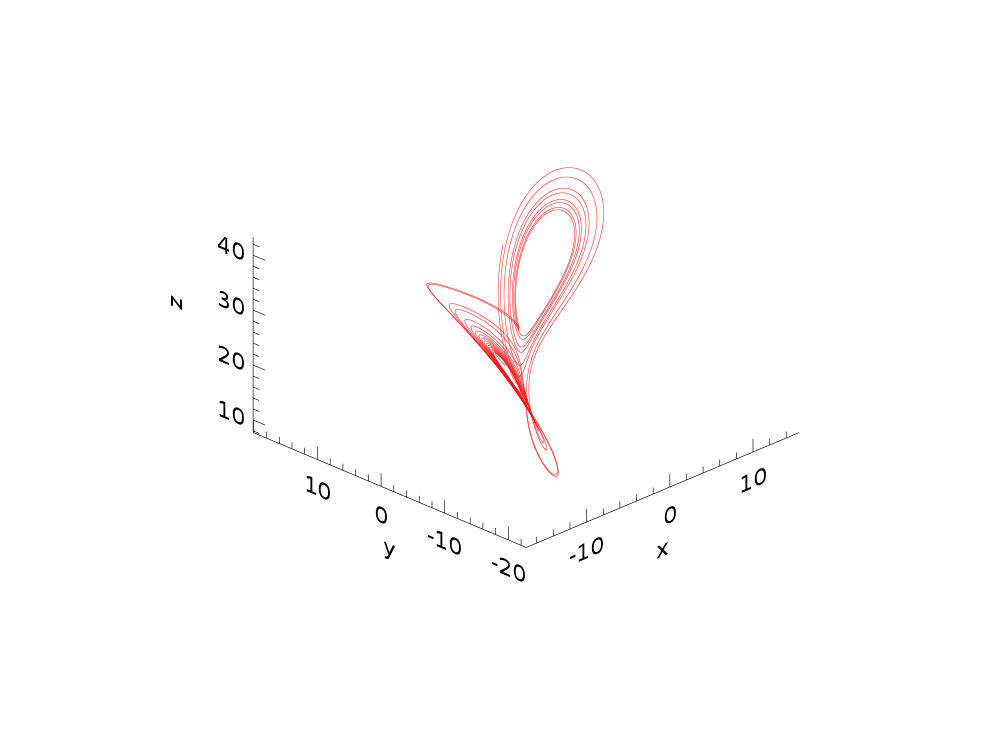
\includegraphics[width=\columnwidth]{plots/3d_sol.png}
\footnotesize{\caption{Solution}}
\end{figure}

\begin{figure}
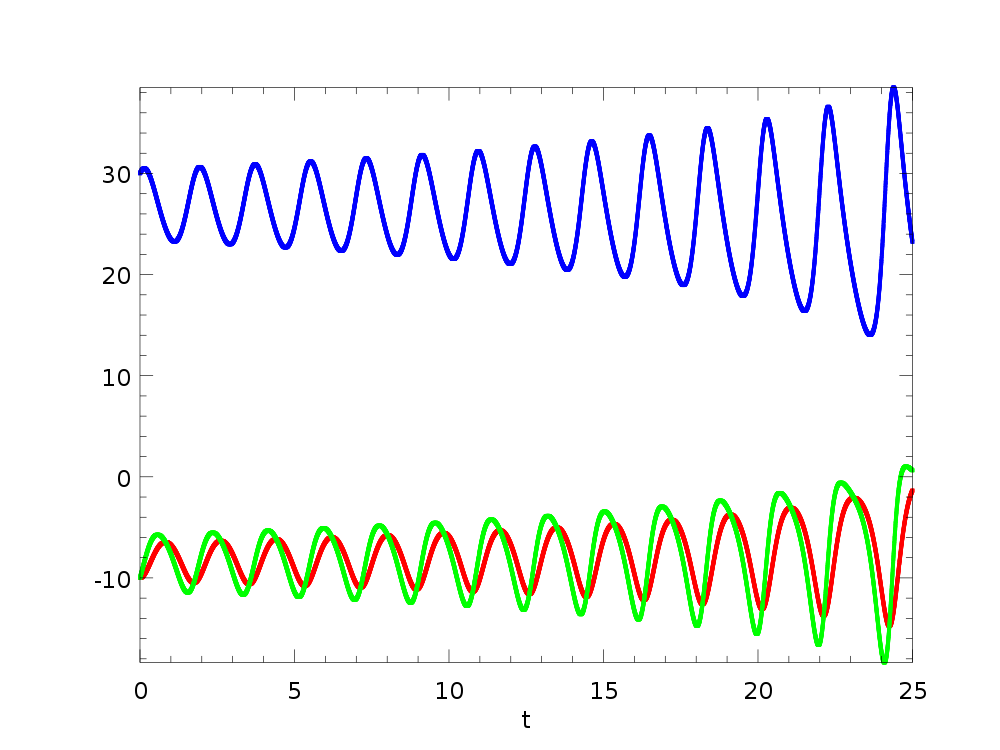
\includegraphics[width=\columnwidth]{plots/xyz_impl.png}
\footnotesize{\caption{Solution vector}}
\end{figure}

\begin{figure}
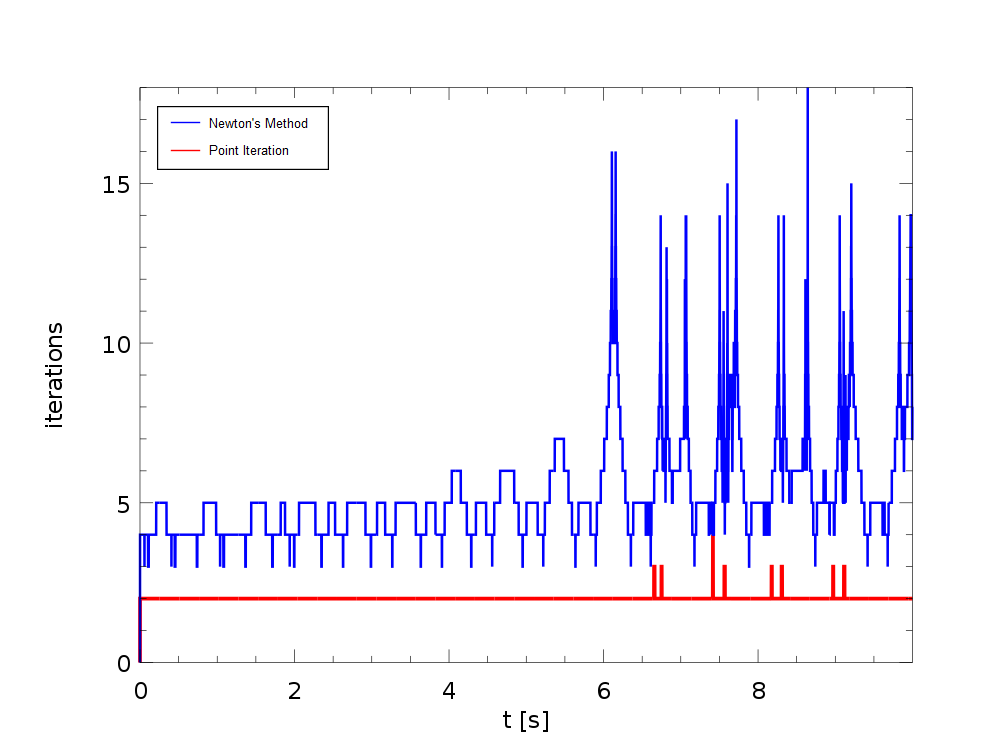
\includegraphics[width=\columnwidth]{plots/iterations.png}
\footnotesize{\caption{Iteration Comparison}}
\end{figure}
\end{document}

